%\documentclass[12pt, a4paper, oneside]{book}
\documentclass[12pt, a4paper, titlepage, twoside]{book}
%\documentclass[a4paper,11pt,twoside]{report}
% TODO: should I change it to report? what is twoside?
\usepackage[latin1]{inputenc}
\usepackage[cyr]{aeguill}

% farzaneh \usepackage[francais]{babel}

\usepackage{fancyhdr, ifpdf}
\usepackage{array}
\usepackage{multirow}
\usepackage[latin1]{inputenc}

%\def\pgfsysdriver{pgfsys-dvipdfm.def}
%\usepackage{tikz}

\usepackage{textcomp}

\usepackage{verbatim} 

\usepackage{listings}
\usepackage{hyperref}
\usepackage[table]{xcolor}% http://ctan.org/pkg/xcolor
\usepackage{hhline}
\usepackage{framed}
\usepackage{pifont}% http://ctan.org/pkg/pifont
\usepackage{tikz}
\def\checkmark{\tikz\fill[scale=0.4](0,.35) -- (.25,0) -- (1,.7) -- (.25,.15) -- cycle;} 
\newcommand{\cmark}{\ding{51}}%
\newcommand{\xmark}{\ding{55}}%
\usepackage{algorithm}
\usepackage{algorithmic}
%\usepackage{amsmath}
%\usepackage{algorithm}
%\usepackage[noend]{algpseudocode}


% Uncomment to show frames
%\usepackage{showframe}

%\setlength{\hoffset}{0.5cm}
\setlength{\oddsidemargin}{1.3cm}
\setlength{\evensidemargin}{0.8cm}

%\setlength{\marginparwidth}{2cm}
  
%Pour montrer les label
%\usepackage{showkeys}
%\usepackage{showlabels}

%\usepackage{varioref}
%\usepackage[french]{varioref} 
\usepackage{booktabs}
\newcommand{\otoprule}{\midrule[\heavyrulewidth]}

\usepackage{amsmath,amssymb,amstext,mathtext}

\definecolor{LightBlue}{rgb}{0.8,0.8,1.0}
% Uncomment one of these line depending whether you want to see the draft or the final version.
%\usepackage[draft]{graphicx}
% TODO: What is a draft?
\usepackage{graphicx}
\graphicspath{{./figures/}{./logo/}}

\makeatletter
\def\cleardoublepage{\clearpage\if@twoside \ifodd\c@page\else
\hbox{}
\vspace*{\fill}
\begin{center}
\end{center}
\vspace{\fill}
\thispagestyle{empty}
\newpage
\if@twocolumn\hbox{}\newpage\fi\fi\fi}
\makeatother

\pagestyle{fancyplain}

% some redefination of the headers and footers
\renewcommand{\chaptermark}[1]%
                 {\markboth{#1}{}}
\renewcommand{\sectionmark}[1]%
                 {\markright{\thesection\ #1}}
\lhead[\fancyplain{}{\thepage}]%
      {\fancyplain{}{\rightmark}}
\rhead[\fancyplain{}{\leftmark}]%
      {\fancyplain{}{\thepage}}
\cfoot{}
\sloppy

% Farzaneh \ifpdf
% Farzaneh   \usepackage[pdftex]{graphicx}
% TODO: do I need this?
%   \pdfinfo {
%      /Title (A monolithic microrobotic arm in silicon)
 %     /Subject (Rapport de projet de semestre)
 %     /Author (Marc Stranczl)
 %     /Keywords (SOI)
 %  }
% Farzaneh \else
% Farzaneh   \usepackage{graphicx}
% Farzaneh \fi



\begin{document}


%% http://en.wikibooks.org/wiki/LaTeX/Title_Creation
% Adjusted for EPFL template


\begin{titlepage}

\begin{center}

\raisebox{2cm}[-2cm][-2cm]{
\hspace{-1.5cm}

  \footnotesize
  \begin{tabular}{@{\hspace{10pt}}l@{\hspace{0pt}} l@{\hspace{10pt}}}
  %  \cline{0-0}     &\multirow{5}{*}{\hspace{10pt}\raisebox{-1ex}{
\includegraphics[width=0.4\columnwidth]{CERN-logo}}}\\
    \multirow{5}{*}{\hspace{10pt}\raisebox{-1ex}{
\includegraphics[height=0.2\textheight]{CERN-logo}}}    & \multirow{5}{*}{\hspace{10pt}\raisebox{-1ex}{
\includegraphics[width=0.4\columnwidth]{EPFL_LOG_QUADRI_Red}}}\\

         \\
    \\
    \raisebox{1.2ex}{INSTITUT DE MICROTECHNIQUE | Laboratoire de Microsyst�mes} \\
    %\scriptsize CH -- 1015 LAUSANNE \\

  \end{tabular}%
}

\vspace{1\baselineskip}
\Huge

\newcommand{\HRule}{\rule{\linewidth}{0.3mm}}


    {\huge \bfseries  A monolithic microrobotic arm \\ in silicon} \\
    {\Large \bfseries  Microrobot monolithique en silicium} \\
	\vspace{3mm}    
    \textsc{\Large Projet de Semestre} \Large (Automne 2009) \\
    \Large Section Microtechnique
    
    %\HRule \\[0.2cm]
	
	\vspace{3mm}
	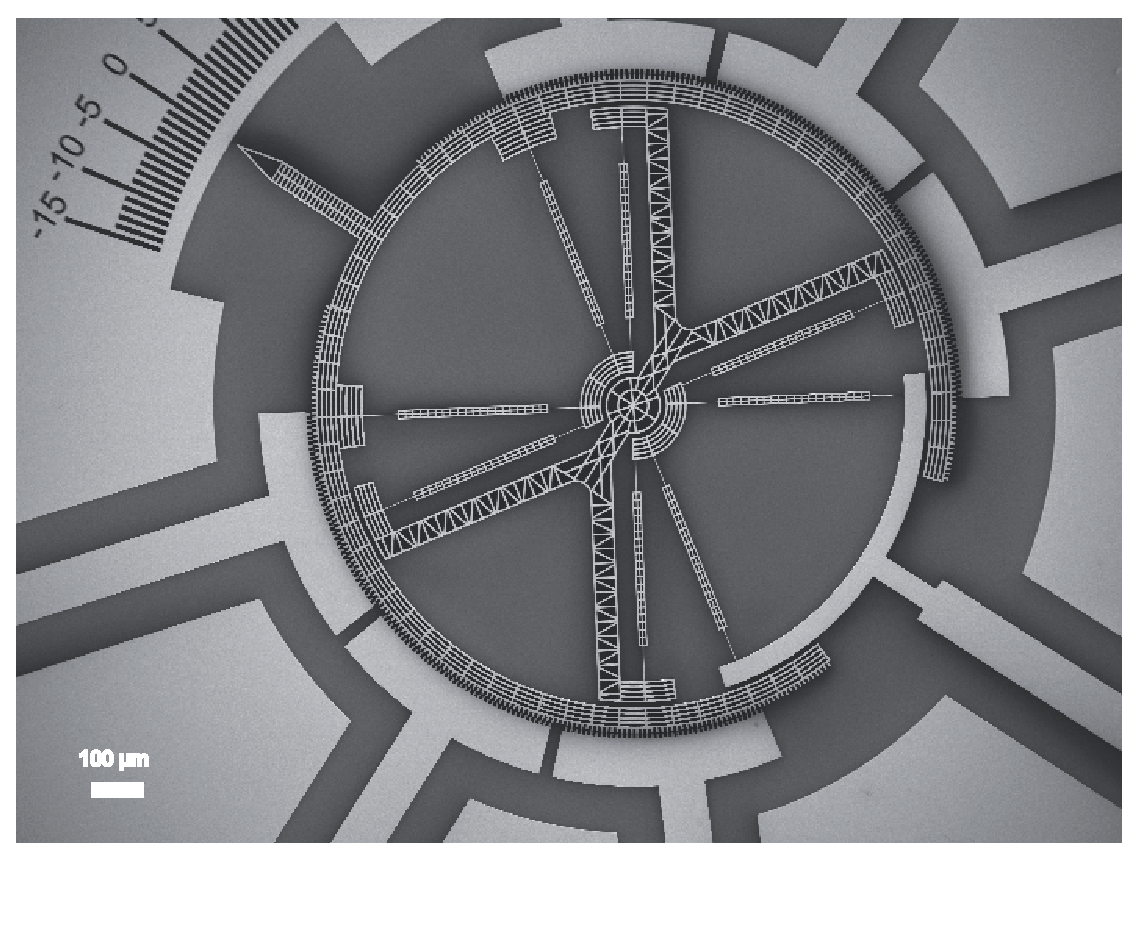
\includegraphics[height=6 cm]{fig_couverture}
	\vspace{3mm}
	\HRule 
	
	\emph{Auteur:} \\
	Marc \textsc{Stranczl}\\
    \vspace{0.5cm}
    \emph{Sous la supervision de:} \\   

    Prof. Martinus \textsc{Gijs}, LMIS2 \\   
    Dr. Christophe \textsc{Yamahata}, LMIS 2\\

	\vspace{0.5cm}
    % Bottom of the page
    \emph{Remis le: 8 janvier 2010}
	%{\large \today}


\end{center}


\end{titlepage}

\newpage
\thispagestyle{empty}
\mbox{}
%\maketitle

%\begin{titlepage}
%\fancyhf{}

% http://en.wikibooks.org/wiki/LaTeX/Title_Creation
% Adjusted for EPFL template


\begin{titlepage}

\begin{center}

\raisebox{2cm}[-2cm][-2cm]{
\hspace{-1.5cm}

  \footnotesize
  \begin{tabular}{@{\hspace{10pt}}l@{\hspace{0pt}} l@{\hspace{10pt}}}
  %  \cline{0-0}     &\multirow{5}{*}{\hspace{10pt}\raisebox{-1ex}{
\includegraphics[width=0.4\columnwidth]{CERN-logo}}}\\
    \multirow{5}{*}{\hspace{10pt}\raisebox{-1ex}{
\includegraphics[height=0.2\textheight]{CERN-logo}}}    & \multirow{5}{*}{\hspace{10pt}\raisebox{-1ex}{
\includegraphics[width=0.4\columnwidth]{EPFL_LOG_QUADRI_Red}}}\\

         \\
    \\
    \raisebox{1.2ex}{INSTITUT DE MICROTECHNIQUE | Laboratoire de Microsyst�mes} \\
    %\scriptsize CH -- 1015 LAUSANNE \\

  \end{tabular}%
}

\vspace{1\baselineskip}
\Huge

\newcommand{\HRule}{\rule{\linewidth}{0.3mm}}


    {\huge \bfseries  A monolithic microrobotic arm \\ in silicon} \\
    {\Large \bfseries  Microrobot monolithique en silicium} \\
	\vspace{3mm}    
    \textsc{\Large Projet de Semestre} \Large (Automne 2009) \\
    \Large Section Microtechnique
    
    %\HRule \\[0.2cm]
	
	\vspace{3mm}
	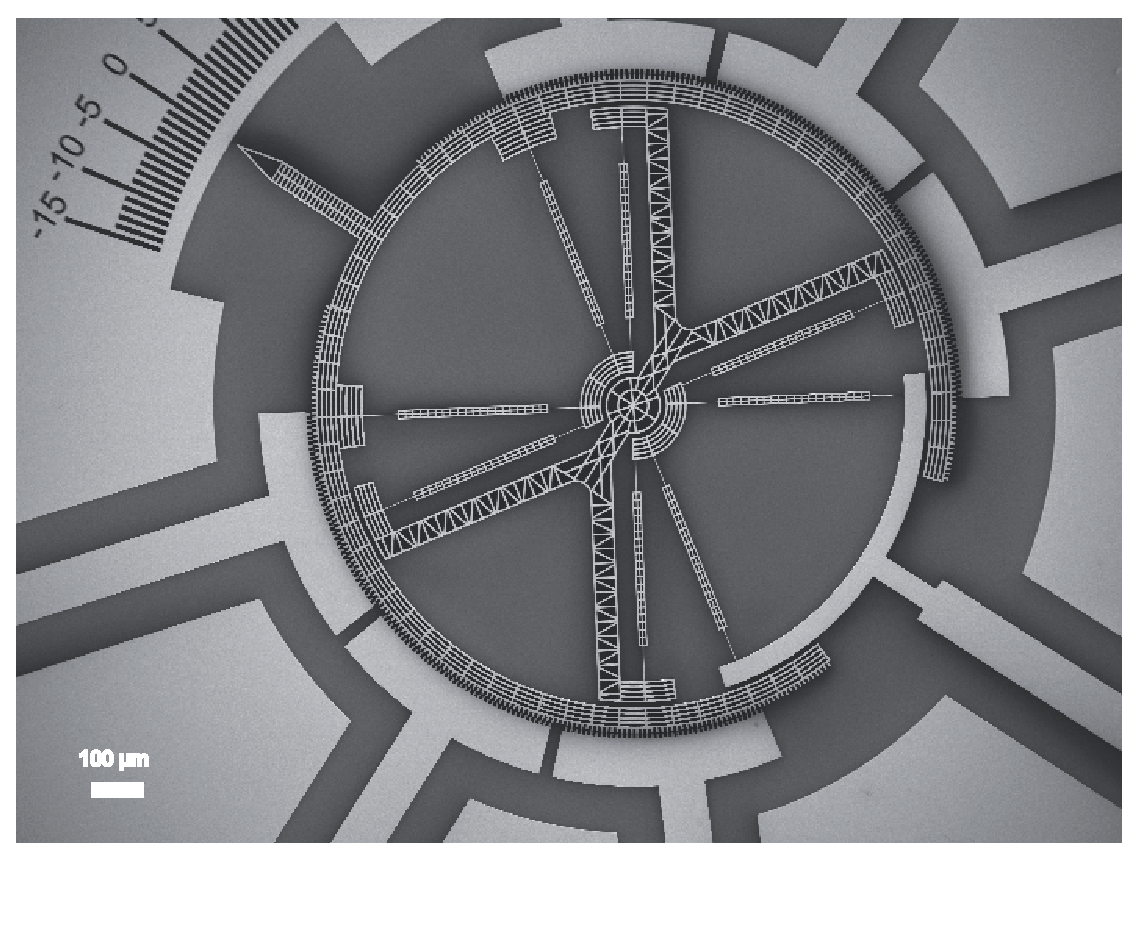
\includegraphics[height=6 cm]{fig_couverture}
	\vspace{3mm}
	\HRule 
	
	\emph{Auteur:} \\
	Marc \textsc{Stranczl}\\
    \vspace{0.5cm}
    \emph{Sous la supervision de:} \\   

    Prof. Martinus \textsc{Gijs}, LMIS2 \\   
    Dr. Christophe \textsc{Yamahata}, LMIS 2\\

	\vspace{0.5cm}
    % Bottom of the page
    \emph{Remis le: 8 janvier 2010}
	%{\large \today}


\end{center}


\end{titlepage}

\newpage
\thispagestyle{empty}
\mbox{}

%\end{titlepage}


%% start the show...
% TODO: I'd rather start it after the table
\pagenumbering{roman}
\setcounter{page}{1}
\pagenumbering{arabic}

\tableofcontents

%\listoffigures
%\listoftables

\chapter*{Abstract}
\thispagestyle{empty}

It is crucial for big organizations like CERN with a very large web landscape to ensure the security of their web resources. One can use various open source or commercial web scanners to scan websites and look for common, well-known web vulnerabilities. However, these scanners usually fail to find vulnerabilities that are discovered every day in software products and commonly used libraries. The main objective of this project is to automate the procedure for detecting vulnerable web applications remotely and when new vulnerabilities emerge. For this purpose, we will introduce a tool that monitors vulnerability sources to find newly discovered vulnerabilities, and detects CERN resources that use vulnerable third party products. In addition, we introduce another tool that facilitates scanning CERN resources for critical vulnerabilities in emergency cases, specially when a vulnerability is not specific to a certain, detectable third party product.

\chapter{Introduction}
\label{introduction}
\thispagestyle{empty}
Over the past decade, web applications have been embraced by many companies to deliver their main services to customers. One can think of different reasons for this increase in popularity: ubiquity of web browsers makes it convenient to use them as a client; web applications can be updated and maintained locally with no need to distribute or install software on the client side and web applications are cross-platform compatible.
Another reason for the increasing popularity of web applications is the simplicity of developing them. Nowadays there are many web application frameworks and content management systems that facilitate rapid application development. This simplicity comes with a cost: securing a web application is difficult. Web applications include code that resides on the web servers, application servers, databases, and back-end systems of an organization. The potential for a security breech exists in each of these layers. This opens the door to attackers trying to manipulate the application logic to perpetrate their misdeeds\cite{secure_web}. In this project, we are going to focus on approaches for maintaining the security of web applications at CERN\footnote{European organization for nuclear research}. CERN is a large particle physics research organization and it manages thousands of websites and web servers for different purposes. Ensuring the security of this large web landscape is one of the main priorities of its Computer Security Team.

\paragraph{}
Even if a web application is designed to be as secure as possible, vulnerabilities will invariably be discovered over time in its code or in the code of underlying packages it uses and relies on. Therefore, to continue ensuring that the application remains secure, it is important to constantly check for newly discovered vulnerabilities and make sure that the application is not affected. This task is easier for the application designers themselves, who are aware of all the technologies that are used in their application; however, in many organizations like CERN, any employee can set up a web server or launch a website and few employees bother to monitor their own web applications for security vulnerabilities. It is the job of the Computer Security Team to scan these various web servers and websites and detect all vulnerabilities remotely.
\paragraph{}
There are two main approaches for ensuring the security of web applications: The first approach is to use the available automatic scanning tools, such as Acunetix or Skipfish\footnote{Google open source security reconnaissance tool}, to detect vulnerabilities. Using this approach, we can find common vulnerabilities, but when a new vulnerability emerges we have to wait for the new version of the scanning tool to be released and include tests for the new vulnerability. Also, due to the complexity of these tools, it is a time consuming task to configure them for a specific scanning purpose. 
\paragraph{}
The second approach is to keep an eye on vulnerability sources, databases, security mailing lists, etc. to get informed about new vulnerabilities as soon as possible. This way we will not miss any critical vulnerabilities. The next step is to use the vulnerability information to detect any vulnerable resources in the organization. 
\section{Project Focus}
The focus of this project is going to be on the second approach, meaning that we are going to propose two new methods of identifying vulnerable resources affected by newly disclosed vulnerabilities or vulnerabilities that common web scanners fail to identify. 
\paragraph{}
The disclosed vulnerabilities regularly appear on different sources, such as mailing lists, databases, forums, etc. These vulnerabilities might be disclosed with a list of affected products, for example; a vulnerability that affects all websites using Drupal Content Management Systems. In Chapter \ref{vulnerability-notification-tool}, we take advantage of publicly available vulnerability sources and describe a tool we developed --Vulnerability Notification Tool-- that first reports all newly disclosed vulnerabilities and in a second step delivers lists of vulnerable components (from vulnerability information) and uses those lists to alert the CERN Computer Security Team about web applications that may be vulnerable as a result of using those components.
\paragraph{}
On the other hand, sometimes the vulnerabilities are not specific to a certain product, e.g. a vulnerability found in a network protocol or an encryption algorithm, or it is impossible with current tools to detect if a resource is using a certain product. Chapter \ref{scanner} introduces a complementary new tool we developed --Scanner-- that facilitates scanning CERN web applications components with simple (home-grown) security tests to detect individual vulnerabilities on potentially affected components. Heartbleed\footnote{Critical OpenSSL vulnerability, discovered in April 2014} is a good example of a case when it was critical to detect vulnerable resources as soon as possible. The vulnerability was not specific to a single detectable product and most organizations had to use their own (or publicly available) scripts to detect the vulnerability and patch the resources.

\section{Vulnerability Definition}
According to the MITRE CVE initiative\footnote{\url{http://cve.mitre.org/about/terminology.html\#Dist}}, a vulnerability is a mistake in software that can be directly used by a hacker to gain access to a system or network. A vulnerability would allow an attacker to:
\begin{itemize}
\item execute unauthorized commands
\item access data that is contrary to the specified access restrictions for that data
\item pose as another entity or user
\item conduct a denial of service
\end{itemize}

Note that a vulnerability can be a result of a mistake in design or in configuration of a product. For example, not changing the default password is a configuration rather than a design vulnerability that will open a door to attackers. 

\section{CERN Web Landscape}
CERN provides different web services, such as web authoring and web publishing for its users. The purpose of the CERN Web-services\footnote{\url{http://cern.ch/web}} is to avoid website duplication and locally managed web servers, as well as proposing standard web authoring technologies. From the security point of view, using web services rather than setting up a locally managed web server is recommended. The people managing the Web-services at CERN are aware of the software used on different layers of the web stack they provide, and if a vulnerability in any of those layers emerges, it is easier to patch the central server, rather than obliging individuals to patch their local web server. However, there is no restriction on setting up a local web server and any employee can host his websites on a local web server. 

\subsection{CERN Websites}
There are more than 13k websites at CERN that are centrally hosted by the CERN Web-services. These websites have a URL in the format of \url{http://cern.ch/X} or \url{http://X.web.cern.ch}, where X is the name of the website. CERN homepage at \url{http://home.web.cern.ch/} is an example of websites that are hosted centrally. When creating a new website the user can choose the type of the website from the following list:
\begin{itemize}
\item \textbf{Centrally Hosted on DFS\footnote{Distributed File System}}: This type is recommended for Windows users. The DFS site is linked to a dedicated DFS folder where the user can edit files as she pleases with any authoring tool she may have.
\item \textbf{AFS\footnote{Andrew File System} Folder}: This type plays a similar role for Linux users. Each AFS site is related to an AFS folder.
\item \textbf{Collaboration Workspace (SharePoint)}: This type is suitable to easily create a collaboration platform to work within teams.
\item \textbf{Social Community}: This type is used to create communities about topics, find answers to questions and connect with others.
\item \textbf{Drupal}: This type provides a Content Management System to publish, edit and organize content through a common web interface.
\item \textbf{Java MiddleWare On Demand site}: This is the type of site for a Java solution for deploying servlets or JSP web applications.
\end{itemize}
The servers hosting these websites are monitored by the CERN Web-services team to stay secure. For example, if a vulnerability in Drupal is discovered the Drupal team will make sure that all Drupal websites are patched immediately. However, each website owner can customize or configure his website to use technologies that might threaten its security. It is the job of the Computer Security Team to scan individual websites and look for vulnerabilities. 
\subsection{Non-central Web Servers}
CERN landscape is not limited to the central web servers and websites hosted centrally by the Web-services. There are more than 1000 instances of dedicated web servers at CERN in the format of \url{http://X.cern.ch} where X is the server name. Indico\footnote{CERN tool for managing conferences, workshops and meetings} at \url{http://indico.cern.ch/} is an example of a dedicated web server. Most of the websites hosted on non-central web servers are only visible inside CERN, but some to have firewall openings and are accessible from the Internet.

\section{CERN Web Security}
The vulnerabilities in web applications can result from three main causes:
\begin{enumerate}
\item A misconfiguration on the server side, such as using weak ciphers or expired certificates, that leaves a door open for attackers
\item Wrong development choices, resulting into cross-site scripting (XSS), etc.
\item Use of Vulnerable third party software, e.g. an outdated Drupal instance, that needs to be updated or patched
\end{enumerate}
The CERN Computer Security Team uses various tools and procedures to prevent exposure of vulnerable web applications to the world outside the organization. Also, it is important to detect any vulnerabilities in web applications as soon as possible and take necessary actions to secure the whole web infrastructure inside CERN.

% Fiesty :-) 
\subsection{Prevention}
In order to lower the probability of developing vulnerable software, users are encouraged to use CERN central Web-services to create websites. In addition, whenever a website is being published on the Internet and is accessible from outside CERN network it has to go through the firewall opening procedure. In the firewall opening procedure, a member of the Security Team analyzes the case completely to make sure that the request is reasonable, e.g. there are enough reasons for not using the central Web-services. Additionally, tools like OpenVas\footnote{Open Vulnerability Assesment System} and Skipfish will be used to scan the website and report the vulnerabilities and warnings back to the owner of the website. 

\subsection{Detection}
Whenever a new vulnerability is published, it is a part of the CERN Computer Security Team job to find affected resources and notify their owners. Currently, the Computer Security Team members get informed about new vulnerabilities by subscribing to product mailing lists, security forums, Twitter accounts, etc. If they decide that a vulnerability is worth investigating the next step is to scan the whole web infrastructure for the vulnerable resources. For this purpose, small detection scripts are developed or downloaded (e.g. Heartbleed vulnerability or ShellShock\footnote{Critical Shell vulnerability discovered in September 2014}). The detection scripts can also look for misconfigurations, such as empty landing pages or HTTP (instead of HTTPS) authentication. 


\section{Relevant Tools}
\label{sec:tools}
\paragraph{}
Typically tools are used by the CERN Computer Security Team to ensure the security of CERN resources. This section gives a short description of the tools that are relevant to this project and are mentioned in the following chapters. 
\subsection{Web Application Scanning} 
The Web Application Scanner (WAS) is a tool that can be used to generate a list of all web servers and websites at CERN, run the Skipfish web scanner on each of the detected URLs and report warnings and vulnerabilities, or run the Web Application Detection (WAD) tool to detect technologies used on a particular website or web server.
\subsubsection{Web Application Detection}
The CERN web landscape - both independant web servers and centrally-hosted websites - are regularly scanned with the Web Application Detection (WAD) tool, in order to detect web applications and technologies they use, and possibly also their versions. This tool is developed using an open source project called "Wappalyzer"\footnote{\url{https://github.com/ElbertF/Wappalyzer}}. Wappalyzer is a cross-platform utility that uncovers the technologies, such as content management systems, eCommerce platforms, web servers, etc. used on websites.  Wappalyzer uses a set of predefined rules to detect technologies and these rules are stored in a JSON file. WAD uses this JSON file to detect technologies at CERN. Figure \ref{figure:indico} illustrates a detection rule used to detect Indico instances. It uses regular expressions to search for the phrase ``Powered by Indico'' on the web page. Alternatively it detects Indico instances by the name of the session variables a website uses. This detection rule was added to Wappalyzer and accepted by its original author.
\begin{figure}[h!]

  \centering
    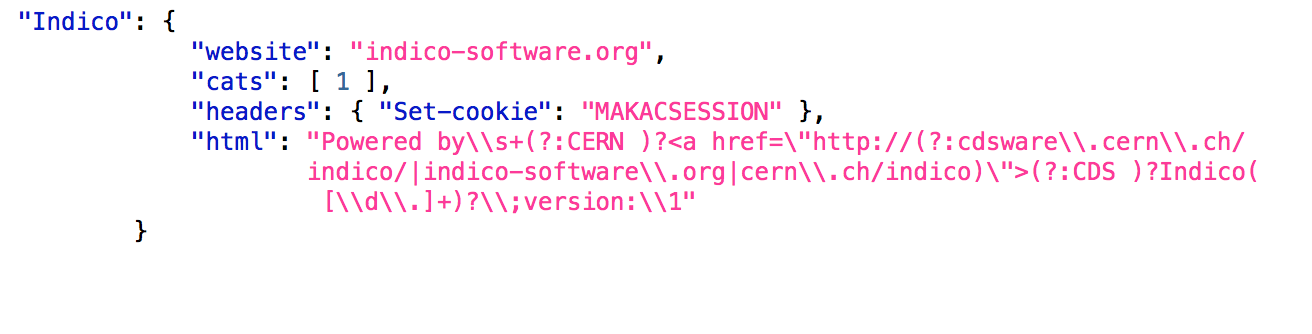
\includegraphics[width=1.0\textwidth]{indico}
  \caption{Indico Detection Rule}
  \label{figure:indico}
\end{figure}
 
\subsection{Detection Scripts}
Over the years, the CERN Computer Security Team has developed individual scripts. Most of these scripts are short security tests to check for an emerging vulnerability (e.g. Heartbleed) on CERN resources. Additionally, some scripts detect misconfigurations (e.g. empty landing pages) on web servers that could threaten the security of CERN resources. Currently, CERN can detect the following vulnerabilities, using detection scripts:
\begin{itemize}
\item \textbf{Heartbleed} - The device is vulnerable to OpenSSL Heartbleed vulnerability
\item \textbf{SSL2 Check}: - SSL version 2 is enabled
\item \textbf{SSL3 Check}: - SSL version 3 is enabled
\item \textbf{Weak Cipher} - The server is using an insecure cipher
\item \textbf{Homepage Check} - The landing page is empty or the default landing page
\item \textbf{CouchDB Check} - The CouchDB\footnote{Apache open source NoSQL database that can be accessed from web} database is protected
\item \textbf{Expired Certificate} - The server is using an expired certificate
\item \textbf{Self-signed Certificate} - The server is using a self-signed certificate
\item \textbf{Non-valid Certificate} - The server is using a certificate that is not valid for the domain
\item \textbf{Non-trusted Certificate} - The server is using a certificate that is not trusted
\item \textbf{Wildcard Certificate} - The server is using a wildcard certificate
\item \textbf{Basic HTTP Authentication} - The website or web server is using Basic HTTP Authentication
\item \textbf{OpenSSL CCS Injection} - The device is vulnerable to the OpenSSL Change Cipher Spec (CCS) injection vulnerability

\end{itemize}



\section{Objectives}
\paragraph{}
The main objective of this project is to automate --as much as possible-- the procedures for detecting vulnerable web applications. We would like to take advantage of publicly available vulnerability sources to detect CERN resources that use vulnerable third party products. Another objective of the project is to facilitate scanning CERN resources for critical vulnerabilities in emergency cases, specially when a vulnerability is not specific to a certain, detectable product. This project focuses on detection of vulnerable web applications remotely, more specifically when a new vulnerability emerges.


























%\chapter{CERN Web Landscape}
\label{cern_web_landscape}
In this chapter I am going to blahblah about CERN web landscape obviously
\thispagestyle{empty}

\section{Travaux de Simon Henein}
\subsection{Conception des guidages flexibles}

\begin{figure}[!ht]
\centering
%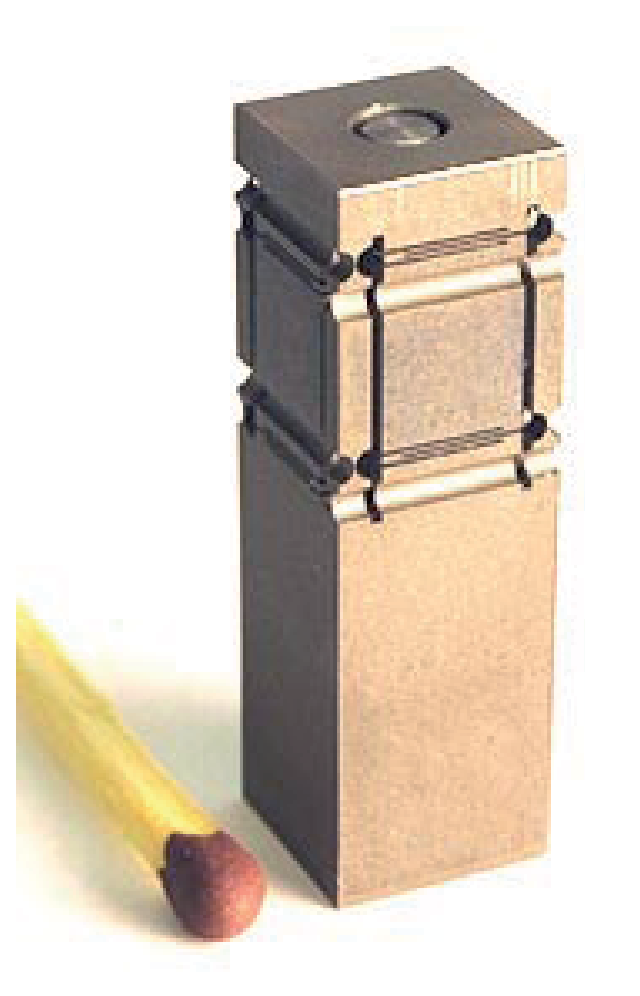
\includegraphics[width=3cm]{figure1.eps}
\caption{figure caption}
\label{fig: image_pivot_fex}
\end{figure}

\newpage

in a new page now
\begin{itemize}
\item first item
\item second item
\item third item
\item fourth item
\end{itemize}

\noindent no indent??


\subsection{Flexure pivot for aerospace mechanisms \cite{henein}}


\begin{figure}[!ht]
\centering
%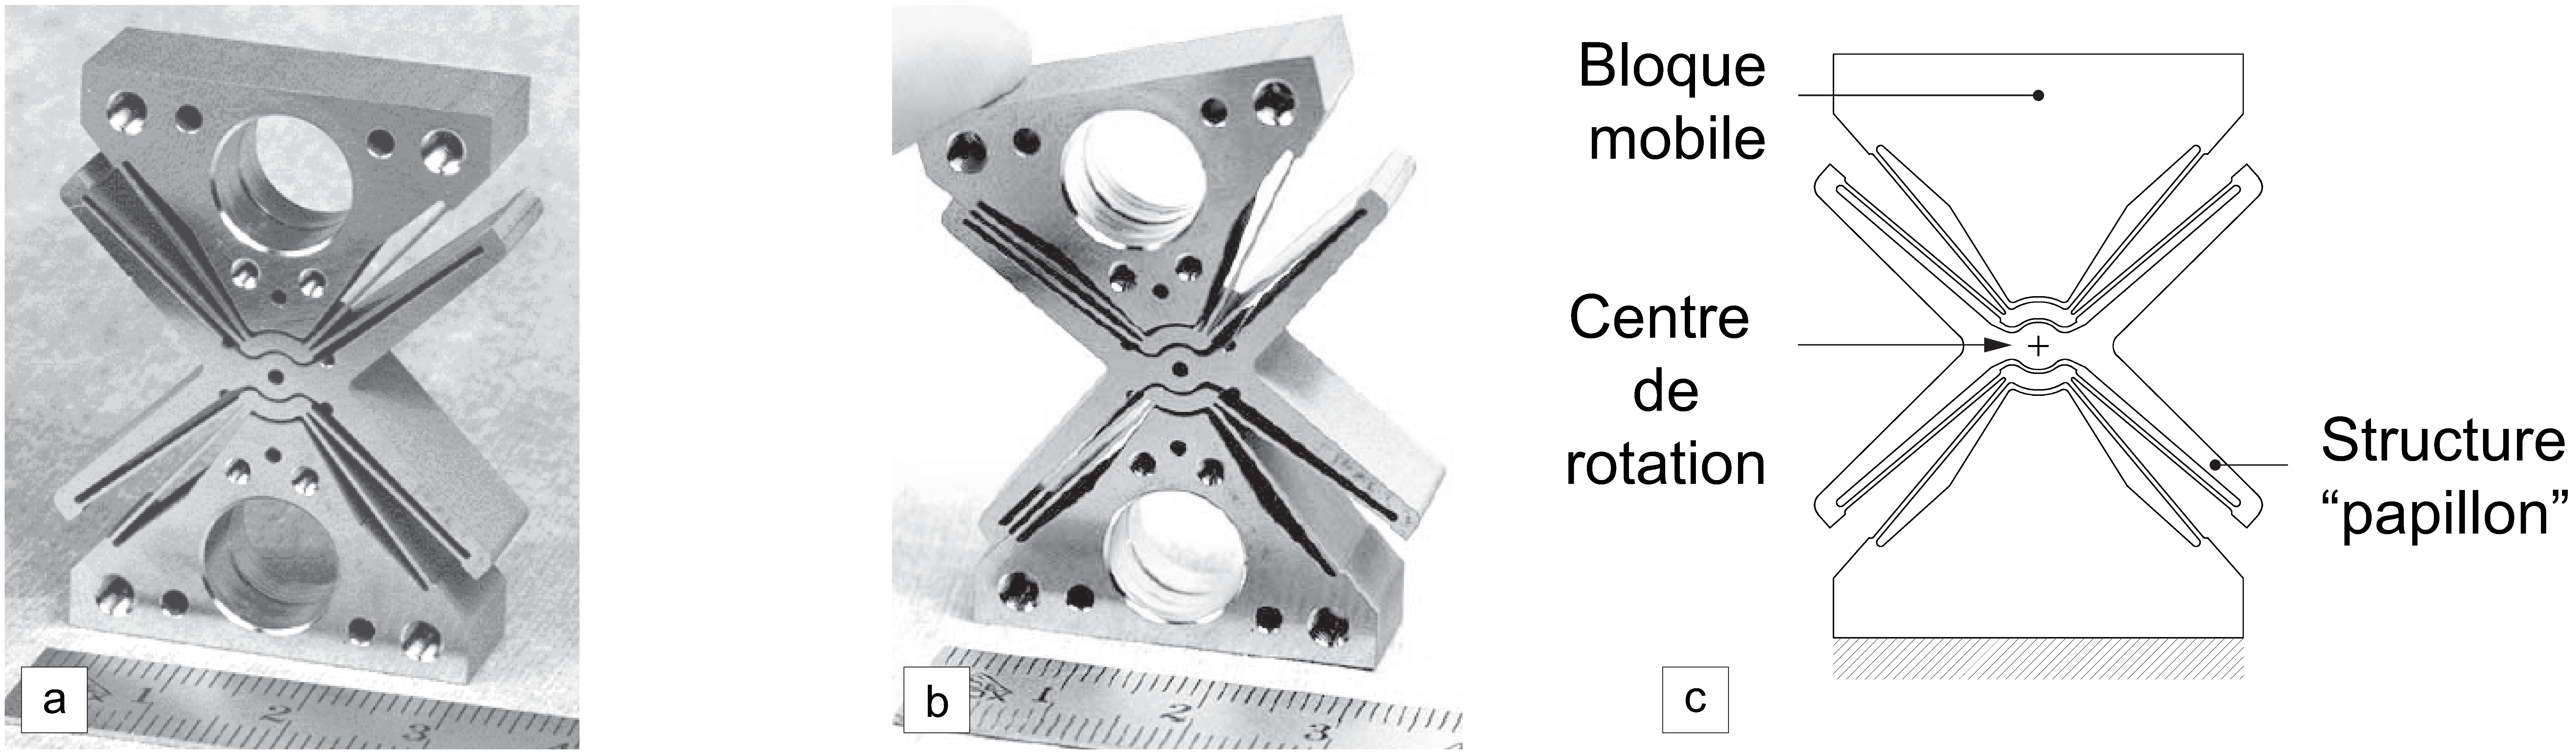
\includegraphics[width=12cm]{figure2.eps}
\caption{Guidage flexible: (a) pivot papillon \ (b) pivot papillon sous contrainte \ (c) something else}
\label{fig: mix_pivot_pap}
\end{figure}

\noindent adasd
\begin{figure}[!ht]
\centering
%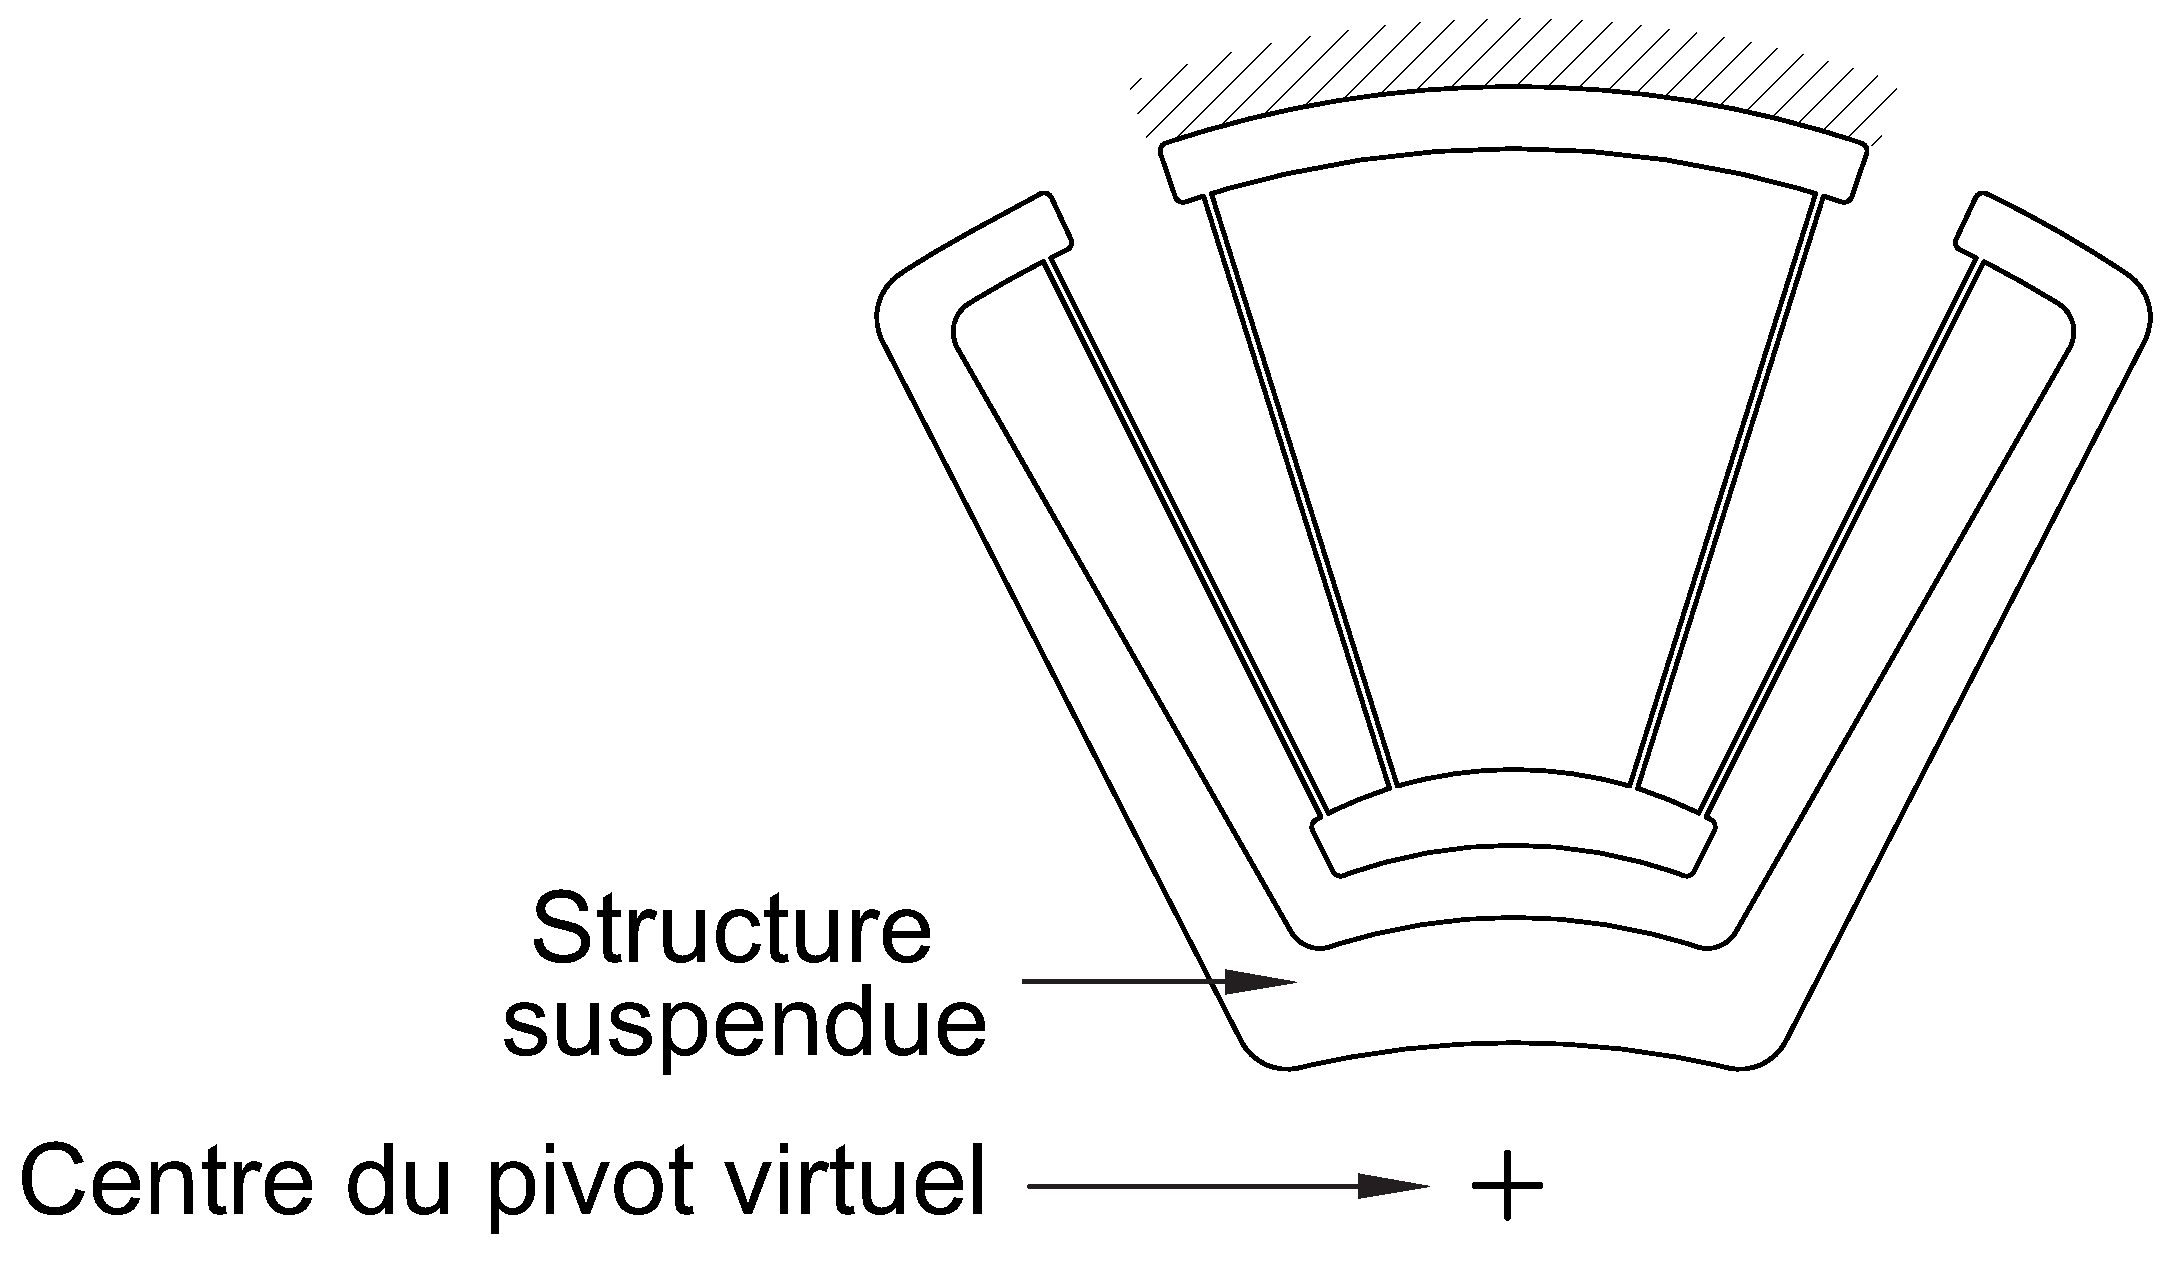
\includegraphics[width=6cm]{figure3.eps}
\caption{Pivot flexible: structure et centre de rotation}
\label{fig: schema_pivot_flexible_art}
\end{figure}




\section{Three-Phase Electrostatic Rotary Stepper Micromotor with a Flexural Pivot Bearing \cite{confidential}}


\begin{figure}[!ht]
\centering
%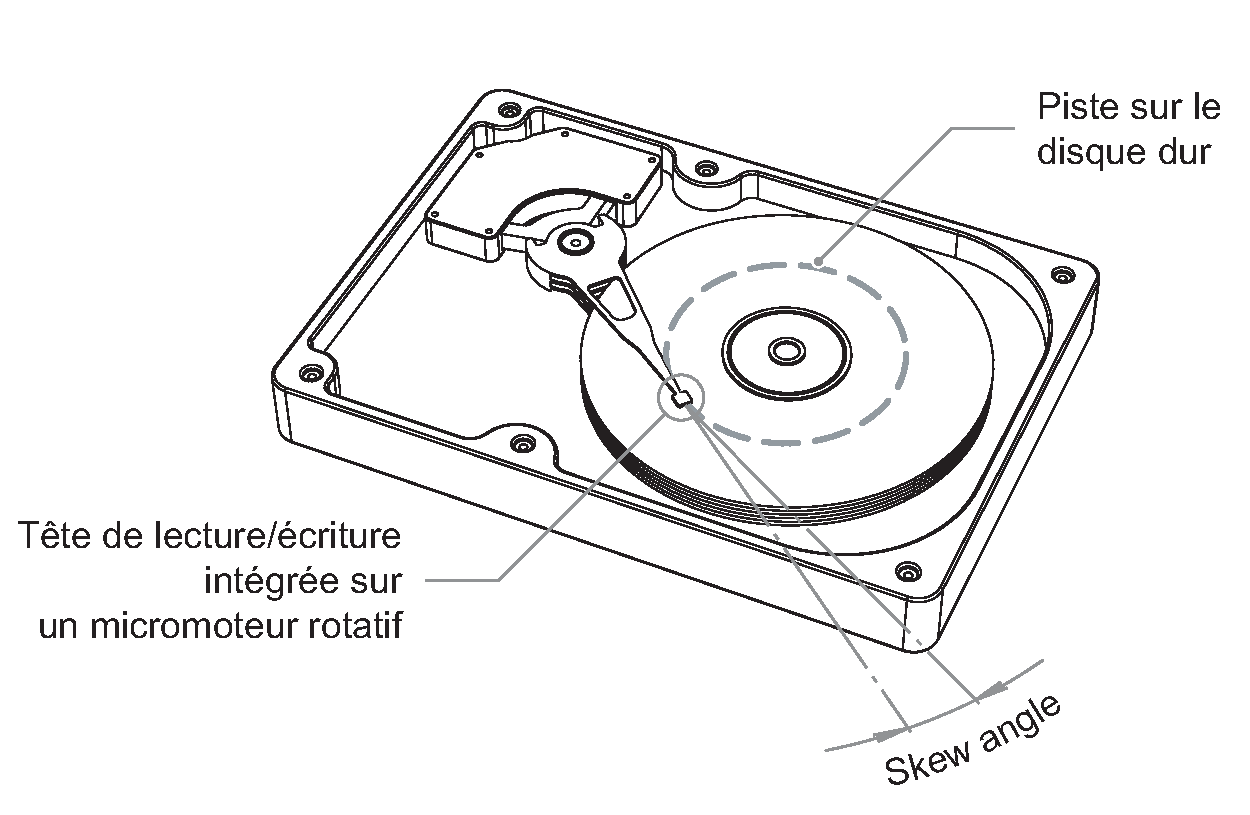
\includegraphics[width=8.5cm]{figure4.eps}
\caption{Disque dur: "skew angle" entre la piste et la t�te de lecture}
\label{fig: schema_HDD}
\end{figure}

\begin{figure}[!ht]
\centering
%\includegraphics[width=12cm]{figure5.eps}
\caption{Moteur:(a) moteur monolithique \ (b) asdasd}
\label{fig: image_moteur_JMEMS}
\end{figure}


\noindent asas
\label{improvements}
\begin{itemize}
\item sdf
\item sdf
\item dsf
\end{itemize}

\noindent sdfsdf

\newpage










\section{Single mask 3-phase electrostatic rotary stepper micromotor \cite{transducers}}


\begin{figure}[!ht]
\centering
%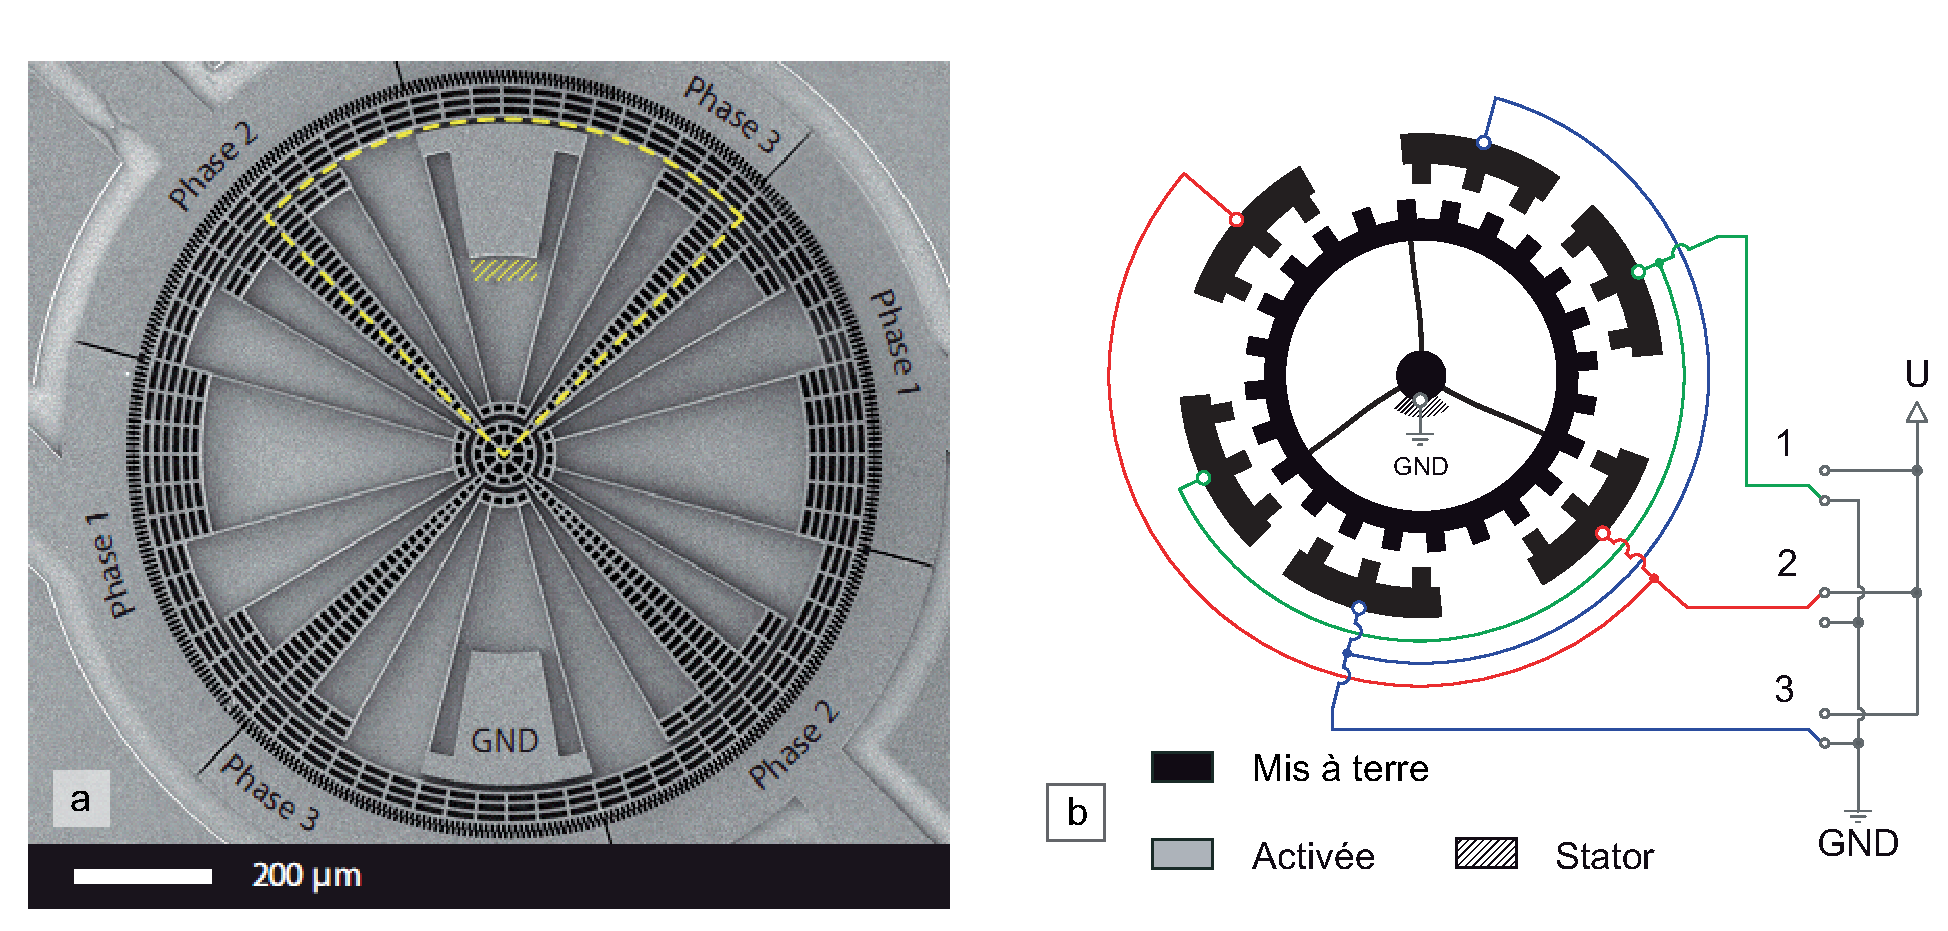
\includegraphics[width=12cm]{figure6.eps}
\caption{Moteur: (a)  moteur monolithique \ (b) asdsad}
\label{fig: image_moteur_edin}
\end{figure}

It's supposed to be funny! 







%\chapter{Vulnerability Detection}
\label{chap3-vulnerability-detection}
\thispagestyle{empty}





\chapter{Vulnerability Notification Tool}
\label{chap5-vulnerability-notification-tool}
\thispagestyle{empty}

\section{Motivation}

Every day new vulnerabilities and security updates are published. Some of these vulnerabilities affect CERN websites/web servers and can be critical, therefore, it is important to learn about them as soon as possible and notify the owners of the affected resources to take necessary actions; i.e., patch their resource. The current procedure in CERN security team for responding to newly published vulnerabilities is as follows:
\begin{enumerate}
\item Getting informed about vulnerabilities from various sources by monitoring public databases, project mailing lists, security mailing lists, twitter accounts, blogs, etc.
\item Deciding if a vulnerability is worth investigating and it might affect CERN (human decision)
\item In case of vulnerabilities related to web applications, the next step is to review the output of WAD on all CERN websites and web servers, in order to get a list of resources that might be affected.
\item Sending notifications to the resource owners after making sure that the resource is in fact vulnerable, i.e runs the vulnerable version or has a vulnerable configuration.
\end{enumerate}

The main goal of the vulnerability notification tool is to automate this procedure as much as possible and optimize each step of the process. 
Staying up to date with vulnerability sources and announcements is a time consuming task and we still do not know if we are monitoring the best sources. Are there other available sources that publish vulnerabilities more quickly with more accurate information and are more complete? With the current procedure we might also ignore some vulnerabilities that are important for CERN, but the public is not talking a lot about them. 
On the other hand there are so many vulnerabilities that are published every day. Figure ????\footnote{\url{http://web.nvd.nist.gov/view/vuln/statistics-results?adv_search=true&cves=on&pub_date_start_month=0&pub_date_start_year=2000&pub_date_end_month=11&pub_date_end_year=2014}} shows the trend in the number of vulnerabilities published in the last 15 years and apparently 2014 with almost 8000 vulnerabilities has been the worst year for security. Due to the ever increasing volume of public vulnerability reports CVE MITRE has even updated the CVE-ID syntax since January 2015, because the previous 4 digit format could only identify at most 9999 vulnerabilities per year.\footnote{\url {https://cve.mitre.org/cve/identifiers/syntaxchange.html}} There is no doubt that it impossible to investigate every single published vulnerability, therefore, it is crucial to filter out the vulnerabilities that do not affect CERN or are not critical in an automatic way.

\section{Related Work}

\subsection{Cassandra}

\section{Source Evaluation}

There are plenty of public sources that announce vulnerabilities or maintain a database of all vulnerabilities over years. The performance of the vulnerability notification tool very much depends on the quality of the source it is using. Obviously it is not possible to find a perfect source as for example there is a trade-off between the speed of publishing the vulnerabilities and accuracy of the information published; hence, It is crucial to know the needs of the organization and choose a source that fits these needs the most.

\subsection{Approach}

In order the evaluate the vulnerability sources the following evaluation factors have been considered:
\begin{enumerate}
\item \textbf{Completeness}: Does the source contain all the vulnerabilities that CERN would probably care about? 
\item \textbf{Speed}: How long since the disclosure of the vulnerability it takes until the vulnerability appears in the source?
\item \textbf{Information Quality}: What information( e.g., severity level, exploits, solutions) about a vulnerability is published on this source?
\item \textbf{Parsable Feed} the source provide parsable feed that can be downloaded/updated automatically?
\end{enumerate} 

A couple of vulnerabilities published over the last few months have been considered to evaluate completeness and speed of different sources. These vulnerabilities were of great importance for CERN and can be a good indicator of how well a source fits CERN needs.
\begin{table}
\begin{center}
    \begin{tabular}{ | c | c | c| }
    
    \hline
    Vulnerability & CVE-ID & Disclosure Date 
    %& Summary 
    \\ \hline
    GitLab groups API & CVE-2014-8540 & 30.10.2015
%     & The vulnerability allows a guest user to delete the owner of a group and to assign any other member as owner through the groups API.
      \\ \hline
    Wordpress 4.0.1 Security Release & CVE-2014-9032(*)  & 20.11.2014
    % & XSS vulnerability allows remote attackers to inject arbitrary web script or HTML via unspecified vectors.[...]\footnote{\url{https://wordpress.org/news/2014/11/wordpress-4-0-1/}} 
    \\ \hline
    Drupal SQL injection
 & CVE-2014-3704
 & 15.10.2014 
 %& The vulnerability allows remote attackers to conduct SQL injection attacks via an array containing crafted keys
  \\
    \hline

 Poodle
 & CVE-2014-3566
 & 14.10.2014
 %& The SSL protocol 3.0 allows man-in-the-middle attackers to obtain clear text data via a padding-oracle attack
  \\
    \hline

Twiki Remote Code Execution
 & CVE-2014-7236
 & 09.10.2014
 %& The debugenableplugins request parameter allows arbitrary Perl code execution.  
 \\
    \hline

ShellShock
 & CVE-2014-6271
 & 24.09.2014
 %& Via certain applications, a local or remote attacker may inject shell commands, allowing local privilege escalation or remote command execution depending on the application vector. 
  \\
    \hline

    \end{tabular}
    \caption{Sample vulnerabilities}
   \end{center}
    \footnotesize{(*) This update fixes multiple vulnerabilities with CVE-2014-9032 CVE-2014-9033 CVE-2014-9034 CVE-2014-9035 CVE-2014-9036 CVE-2014-9037.}
\end{table}


now talk about the sources you considered and at the end the comparisons in the table format. 
\begin{enumerate}
\item \textbf{Drupal SQL injection vulnerability}
\item \textbf{Poodle}
\item \textbf{Twiki remote code execution}
\item \textbf{ShellShock}
\end{enumerate}

\section{National Vulnerability Database}
\subsection{CVSS}
\subsection{Challenges}
\subsubsection{Modification Date}
\subsection{and/or configuration}

\section{Product Name Matching}
\subsection{Common Platform Enumerations}
\subsubsection{Challenges}
completeness
\subsection{WAD Product Names}
\subsection{Matching Algorithms}
\subsection{Evaluation of Algorithms}
Precision and recall?
\section{Notifications}





\chapter{Scanner}
\label{chap4-scanner}
\thispagestyle{empty}

\section{Motivation}

\paragraph{}

Security Team performs scans of various types of resources, such as devices, web servers, web sites. As already discussed in chapter \ref{introduction}, it is impossible to scan these resources manually and there is a need for an Scanning Engine that would facilitate scheduling and running these scans (in both synchronous and asynchronous modes), sharing the load across multiple scanning hosts in a fault-tolerant way, and combining results.
WASDOM as discussed in section \ref{sec:tools} contains various scripts for detecting misconfigurations, e.g. expired certificates, basic HTTP authentication; or for detecting vulnerabilities, such as Heartbleed\footnote{Critical OpenSSL security bug disclosed in 2014}. The scanner as we are going to describe in this chapter is a wrapper around all these short scripts and it aims to facilitate scheduling and running these scripts (scans) by
\begin{enumerate}
\item Enabling the permanent and automatic scanning of resources, i.e. devices, websites, web servers, etc.
\item Making it possible to activate a subset of available detection scripts on targets
\item Showing a list of available detection scripts with an explanation of what kind of detection each does
\end{enumerate} 

\subsection{Use Cases}
\begin{itemize}
\item manual execution
\item automatic execution
\end{itemize}

\section{Scanner Specifications}

\subsection{Plugin Specifications}
\subsection{Resource Types}
\subsection{Scanner Options}
\subsubsection{Examples}

\section{Implementation}
\section{Results}
Is there any?




%\chapter{Evaluation and Results}
\label{chap6-results}
\thispagestyle{empty}

\section{Evaluation}

\subsection{Approach}
simulation of the tool from 31-10-2014 
In order to evaluate the performance of the current tool, two approaches were taken:
\begin{itemize}
\item What vulnerabilities did CERN look into during this time? How fast my tool would find these vulnerabilities?
\item What vulnerabilities were found by my tool and could be important but was missed at CERN? (benefit of using my tool)

\subsection{sending emails}
limiting the number of emails. how to decide? looking over the past two/three month
number of vulns / affected/ critical, etc.

there are many changes in the vulns. I loooked at the kind of changes 

among the changed vulnerabilities from 01.11.2014 to 07.01.2015
\begin{lstlisting}
cat *.txt | cut '-d;' -f1,5,6,8,9 | grep  '^c'|grep -f /afs/cern.ch/user/s/slopiens/public/wad_names_at_cern.txt | grep ';\([6-9]\|10\)\.'  | cut '-d;' -f5  | sed -e "s#\(.*\)\$\$\$\(.*\)#\1\n\2#" | cut -d "%" -f 1| sort | uniq -c
cat *.txt | cut '-d;' -f1,5,6,8 | grep  '^c'|grep -f /afs/cern.ch/user/s/slopiens/public/wad_names_at_cern.txt | grep ';\([6-9]\|10\)\.'  | cut -d ';' -f 2 | sort > vulns-cern-critical-changed.txt
cat *.txt | cut -d ';' -f1,5,9 | grep '^c'|grep -f vulns-cern-critical-changed.txt.ignore | cut -d ';' -f3 |sed -e "s#\(.*\)\$\$\$\(.*\)#\1\n\2#"| cut -d '%' -f 1 | sort | uniq -c
 38 all
 48 cvss_score
 2 description
 304 products
----------------------------------what kind of changes
field%old-value
38 all%unknown
48 cvss_score%None
48 products%
\end{lstlisting}

and decided to ignore version changes in cpe(s) and came up with these new numbers

decsion: send an email to SEC for each vulnerability. either new or changed


if this does not work

vulnerability openstack (CVE-2014-9493) can be an example.
\end{itemize}


\chapter{Conclusion and Future Work}
\label{conclusion-and-future-work}
This project introduced two new tools for detection of vulnerable web applications deployed in a large IT installation. The approaches used in these tools are different from common web scanners, such as Skipfish. In this project we focused more on detecting vulnerable applications as soon as possible by monitoring publicly available vulnerability information. Once we are aware of a vulnerability, we can take two approaches to detect applications that may be a subject to it. If the vulnerability is specific to a software or product, VNT described in Chapter \ref{vulnerability-notification-tool} will report the resources (applications) that use those products. In other cases when the vulnerability is not specific to one product but to its configurations, e.g. an expired certificate, or when detecting the vulnerable technology on resources or applications is not possible or efficient, e.g detecting technologies not supported by WAD, the Scanner (Chapter \ref{scanner}) can be used to run other detection scripts. In addition, the Scanner can be used to run automated regular scans of the whole web infrastructure at CERN and analyze the scan results automatically. Both of these tools are currently being used at CERN to enhance the vulnerability management process of web applications, but there is a potential for improvements in both of them. 
 
\section{Vulnerability Notification Tool}
VNT can be used to get informed about all vulnerabilities, regardless of the product they affect or whether they are web-related. At the moment, it stores all these findings in parsable files. Therefore, it can become a part of the overall CERN vulnerability management mechanism to help keep track of vulnerabilities anywhere. It is possible to extend VNT and evolve it into a vulnerability management framework, where users can decide to ignore some vulnerabilities or get different notifications based on the type of the changes that happen in a vulnerability.
\paragraph{}
The performance of VNT is highly dependent on the vulnerability source it is using. At the time of this project, it was decided to use NVD,  but it is important to keep an eye on the market and use other sources instead of --or along with-- NVD, if they fit the needs described in Section \ref{source_evaluation}. 

\paragraph{}
One of the main challenges while using NVD as the vulnerability source, was the randomness of CPE names. Although CPE is introduced as a standard way of enumerating platforms, there are still many problems with it: Its dictionary is incomplete and contains redundant entries, such as multiple CPE names for the same product. On the other hand, it seems that the available vulnerability sources have not agreed on a standard way of listing vulnerable softwares and each has come up with its own format. The CPE name mapping algorithm described in Section \ref{name_matching} has been tested on NVD CPE data, but would probably be efficient enough on other naming formats with some minor changes. In any case, there seems to be a need for a standard product naming format that is complete and robust enough to meet the requirements of all interested parties. 

\paragraph{}
The product name matching algorithm that is currently being used to find vulnerable products can also be improved. In addition to application names, WAD provides the category (type) of each application. The current algorithm described in Section \ref{name_matching} ignores the category of WAD names. A possible improvement to the algorithm would be to report matches only if the CPE type (first field of the CPE name) and WAD category match (e.g. both are operating systems). Another potential improvement is to use available algorithms for computing the string distance between CPE and WAD names, reporting only the pairs that have a similarity higher than a decided threshold.  

\paragraph{}
Alternatively, WAD can be extended to include the equivalent CPE name(s) for each WAD name. This approach can ensure a higher accuracy level, because there will be no need for a name matching algorithm. However, maintaining this dictionary of WAD names to CPE names will be necessary whenever new WAD names are added to WAD. Ideally, this extension can be done to Wappalyzer to benefit from the community of Wappalyzer to maintain the dictionary. But Wappalyzer does not have a security purpose and it would be a challenge to convince its community to care for finding equivalent CPE names whenever they add a new detection rule (with a new WAD name). 

\paragraph{}
NVD reports a list of affected product versions, but this data changes very often. One can notice that previously announced vulnerable versions sometimes get removed from NVD updates or versions that were not reported as vulnerable, enter the list. There are many cases where vulnerability information gets updated on NVD with a small change in the sub-sub-version of an affected product. If VNT was sending update notifications for every change in affected product versions, it would flood its users with updates, encouraging them to ignore such notifications completely. Therefore, in the current tool, we decided to ignore any changes in product versions. Apparently, knowing about these changes can be useful in some cases though. Imagine that there is a vulnerability that is affecting Drupal version 6. We might decide to ignore this vulnerability at CERN, because all Drupal instances are using version 7 or higher. If a couple of days later, NVD updates the same vulnerability and lists Drupal 7 as a vulnerable product, we would definitely like to receive an update notification. As one can see, there is a trade-off here and it can be an open question to the CERN Computer Security Team to decide if they would rather receive more notifications (among which many are useless), for the sake of not missing important product version changes in vulnerability information.
\paragraph{}
For the time being, VNT is sending email notifications to the CERN Computer Security Team members rather than the resource owners. The reason is that, in most cases, further investigation of a vulnerability is needed to make sure that the reported resources are indeed affected. One step towards fully automating the tool is to consider product versions when reporting the resources.
\paragraph{}
The product version reported by WAD, however, is not always reliable. For instance, Apache servers might be reported to have obsolete versions while the new updates have been back-ported\footnote{Parts of a newer version of a software have been added to an older version of the same software, without upgrading.} to them. In addition, WAD is unable to detect the version of many products, e.g. CakePHP framework. Due to these limitations, it was decided to ignore product versions when reporting vulnerable resources and leave it to the investigator of the vulnerability to decide if a certain resource is indeed affected. Once WAD supports more reliable version detection, VNT can be slightly changed to only report resources that use a certain version of a product.
\paragraph{}
Used in a slightly different way, VNT can be used to make sure that new resources at CERN are not vulnerable. Whenever there is a new resource detected by WAD, we can use VNT data to ensure that this new resource is not vulnerable to recently found vulnerabilities.
\section{Scanner}
The Scanner facilitates running individual detection scripts on CERN resources. Currently, it supports detection scripts that run on websites and web servers (devices). It can be easily extended to support other types of resources at CERN. For example, CERN is managing user accounts and each of these accounts can be considered as a resource. Each account is associated with an AFS space and one can think of scanning all accounts at CERN to find out if a user is storing his private keys in an AFS public folder. This would be a security risk for the user, because everyone in the organization would have access to his private key. The Scanner could be used to run this script on all accounts at CERN if provided with relevant inputs to pass into the detection script.
%% change the example: for example talk about checking public / private key available on AFS
%a password has been exposed (when a list of exposed email addresses and passwords is advertised publicly) and write a detection script for this purpose. 
\paragraph{}
Currently VNT and the Scanner are two separate tools for different purposes. In cases that a vulnerability detected by VNT needs further investigations, it would be valuable to connect VNT to the Scanner. This could help the CERN Computer Security Team test for themselves whether a given server or site is actually subject to a VNT-reported vulnerability by writing a corresponding plugin and launching the Scanner to check the VNT-reported targets, then automatically trigger a mail notification if the vulnerability is confirmed.


\bibliographystyle{unsrt}
\addcontentsline{toc}{chapter}{Bibliographie}

\nocite{*}

\thispagestyle{empty}
\bibliography{bibliographie}

\begin{appendix}
\appendix
\chapter{Annexes}
\label{app}


\section{Conception des masques}
\label{masque}



Le tableau \ref{masque} regoupe les dimensions du masque et les dimensions pr�vues .

\begin{table}[!ht]
\renewcommand{\arraystretch}{1}
\centering
\begin{tabular}{l r r }
\toprule
\textbf{}					&\multicolumn{2}{c}{\textbf{Dimensions}} \\ 
\textbf{Param�tres} 					& \textbf{sur masque}	& \textbf{sur wafer} \\
\midrule
Largeur des lames souples			& $3\mu m$ 				& $2.5\mu m$ 	\\
Largeur des lames rigides			& $2.5\mu m$ 			& $2  \mu m$ 	\\
Largeur d'une dent large			& $5 \mu m$				& $4.5 \mu m$	 \\
Largeur d'une dent �troite			& $4 \mu m$				& $3.5 \mu m$	 \\
Gap (rotor/stator)					& $1 \mu m$				& $1.5 \mu m$ 	 \\
\midrule
Largeur des lames du robot v 2.5	& $2.5\mu m$ 				& $2\mu m$ 	\\
Largeur des lames du robot v 2.0	& $2.0\mu m$ 				& $1.5\mu m$ 	\\
Largeur des lames du robot v 1.5	& $1.5\mu m$ 				& $1\mu m$ 	\\
Largeur des lames du robot v 1.0	& $1.0\mu m$ 				& $0.5\mu m$ 	\\
\bottomrule
\end{tabular}
\caption{Dimensions des param�tres sur le masque de la deuxi�me verison et dimensions pr�vues sur wafer}
\label{table:masque}
\end{table}

La fabrication et la mise au point du processus de fabrication a �t� donn� � une personne externe. Le lecteur est invit� � se r�f�rer aux annexes \ref{process flow} et \ref{runcard} pour le processus en lui-m�me.

\section{Constantes physiques et propri�t�s des mat�riaux}
\label{constantes}

Les valeures suivantes ont �t� utilis�es pour les applications num�riques. Afin de s'affranchir des propri�t�s anisotropes du silicium, les valeurs les plus contraignantes de ces propri�t�s ont �t� consid�r�s. Un coefficient de s�curit� de 10 a �t� pris pour les contraintes admissibles maximum.

\begin{table}[!ht]
\renewcommand{\arraystretch}{1}
\centering
\begin{tabular}{lcr@{}l}
\toprule
\textbf{Param�tres} 			& \textbf{Symboles}	& \multicolumn{2}{c}{\textbf{Valeurs}} \\
\midrule
Module de Young					& $E$				& $160$				& $GaOP$ \\
Contrainte admissible 			& $\sigma_{adm}$ 	& $7\times 10^8$ 			& $ Nm^-2$ \\
Permitivit� de l'air 			& $\epsilon$ 		& $8,85\times 10^-12$ 		& $C^2 N^-1m^-2$ \\
\bottomrule
\end{tabular}
\caption{Constantes physiques et propri�t�s des mat�riaux}
\end{table}

%http://fr.wikipedia.org/wiki/Th%C3%A9orie_des_poutres




\section{Contenu du CD-ROM}
\label{cd}


Le CD-ROM contient les fichiers suivants:

\begin{itemize}
\item $Latex$: Rapport du projet de semestre.
\item $Matlab$: Programme de traitement d'image pour mesure dynamique.
\item $Labview$: Programme de commande du micromoteur.
\item $process flow$: Processus de fabrication
\item $runcard$: Protocole du processus de fabrication.
\item $solidworks$: Conception assist�e par ordinateur du moteur.
\item $Cl�win$: Masques sous format .cif
\item $microscopie MEB$: Image prise par Microscopie Electronique � Balayage MEB.
\item $Excel$: Traitement des r�sultats.
\end{itemize}





\section{Processus de fabrication}
\label{process flow}





\section{Protocole du processus de fabrication}
\label{runcard}





\section{Article en cours d'impression: ``Three-Phase Electrostatic Rotary Stepper Micromotor with a Flexural Pivot Bearing''}
\label{annexe_confidential}




\section{Article de la conf�rence Transducers 2009: ``Single mask 3-phase electrostatic rotary stepper micromotor''}
\label{annexe_transducers}







\end{appendix}

\end{document}






